\documentclass[fleqn,10pt]{wlscirep}
\usepackage[utf8]{inputenc}
\usepackage[T1]{fontenc}

% ==== TODO(author): fill in real title/authors/affiliations before submission ====
\title{Predicting Next-Night Sleep Quality from Daytime Wearable Physiology and Activity: A Single-Subject (N-of-1) Machine-Learning Study}

\author[1,*]{Amila Snagić}
\affil[1]{Faculty of Electrical Engineering (ETF), University of Sarajevo, Sarajevo, Bosnia and Herzegovina}
\affil[*]{asnagic1@etf.unsa.ba}

%\keywords{sleep quality, heart-rate variability, wearables, N-of-1, Random Forest, LSTM, explainable AI}

\begin{abstract}
Consumer wearable devices offer a non-invasive route to monitoring sleep, but whether daytime physiology and activity can forecast the quality of the following night's sleep in a single individual remains uncertain. We conducted a retrospective, single-subject (N-of-1) study using five months of consumer wearable exports (124 complete person-days). Each day's heart-rate variability, heart rate, blood-oxygen saturation, step count and energy expenditure were expressed relative to a personal seven-day rolling baseline and, together with same-night sleep latency, used to predict three sleep outcomes: sleep efficiency (Sleep Time Ratio), deep-sleep duration and wake-after-sleep-onset. Random Forest and Long Short-Term Memory (LSTM) models were trained with a strictly chronological design and evaluated once on a held-out test set with bootstrap confidence intervals. Sleep efficiency was predicted with modest but reliable accuracy (Random Forest $R^2 = 0.29$; mean absolute error $\approx 3$ percentage points), whereas deep-sleep duration and fragmentation were not predictable (negative out-of-sample $R^2$). Feature-attribution and lagged-correlation analyses indicated that sleep latency, rather than autonomic physiology, drove the efficiency prediction, and that heart-rate variability did not precede poor or fragmented sleep at any lag up to one week. The Random Forest consistently outperformed the LSTM, consistent with its greater stability in low-sample regimes.
\end{abstract}

\begin{document}

\flushbottom
\maketitle
\thispagestyle{empty}

\section*{Introduction}

Modern society has been characterized by immense technological advancements, revolutionizing all segments of daily life. In such a fast-paced world we often find ourselves straying away from basic human necessities such as sleep. Besides the 7 to 9 hours of sleep typically required by most adults (\url{https://www.sleepfoundation.org/how-sleep-works/sleep-facts-statistics}), many other components play a role in ensuring those hours are composed of good quality sleep. Although sleep quality is a common term in medicine and healthcare, it lacks an established definition as it comprises both objective and subjective criteria. However, this paper will focus on the quantitative measures for establishing sleep quality such as continuity, how much time in bed is actually spent sleeping, and sleep architecture, disruption of deep and REM stages. Sleep ratio, referring to sleep efficiency, is the priorly mentioned ratio between time spent in bed and actual sleep, whereas deep sleep duration is the third stage of non-REM sleep in which the body reaches its highest degree of relaxation, and breathing and pulse become slow and steady. Since the sleep cycle contains 4 phases, it is vital to get enough uninterrupted sleep, thus allowing the body to spend an appropriate amount of time in deeper stages that are essential for physical restoration (energy, cell regeneration, strengthening the immune system, promoting tissue and bone growth and repairment) and cognition (memory consolidation).

Moreover, sleep is closely related to the autonomic nervous system (ANS) which is part of the peripheral nervous system that handles unconscious physiological tasks such as heartrate, digestion and respiration. There is an established bidirectional relationship between sleep and autonomic activity, though the mechanism underlying it remains unclear (\url{https://pmc.ncbi.nlm.nih.gov/articles/PMC7278032/}). We know that different stages of sleep directly impact physiological processes like heart rate which is the slowest and steadiest during deep sleep, however the question remains whether daytime physiological and behavioral metrics may be used as an early non-invasive way to predict quality of sleep. We are looking at the direct relationship between the 2 although there exist many other confounding factors like stress that directly impact the nervous system. When it comes to monitoring vitals, ECG (electrocardiogram) has been the dominant cardiac monitoring technique, but lacks user flexibility, portability and convenience. Therefore, the use of PPG technology has been recognized as an alternative way of providing information about the cardiovascular system. Photoplethysmography (PPG) based technology, such as watches and rings, has become increasingly popular due to its simplicity and efficiency. Such devices can monitor heart rate (HR), heart rate variability (HRV), blood-oxygen saturation (SpO$_2$) and consequently sleep tracking, and activity (steps, calories). These are precisely the metrics recorded in the dataset used for this paper, along with a sleep dataset composed of 3 sleep stages (REM, light and deep sleep), sleep ratio and time asleep as well as time spent awake during sleep stages. Since the same autonomic system governs the transition into and maintenance of sleep, daytime HRV has been proposed repeatedly as an early, non-invasive marker of subsequent sleep disruption. A cross-sectional study examining the relationship between HRV and sleep linked high and very low HRV to poorer self-reported sleep quality and daytime dysfunction across the sample of 60 healthy adults (\url{https://pmc.ncbi.nlm.nih.gov/articles/PMC9103972/#sec5-ijerph-19-05770}). Furthermore, the most directly comparable to the present design, Lee et al. (2025) trained ARIMA, Random Forest, XGBoost, GRU, TCN, Transformer and LSTM models on seven days of preceding HRV, step-count and questionnaire data from 82 participants to predict next-day wake-after-sleep-onset, and reported that the LF/HF ratio was the most informative HRV feature, with deep-learning sequence models providing the best fit given a much larger sample and multi-week windows. A complementary line of work has combined HRV with skin temperature in classifiers of Pittsburgh Sleep Quality Index categories, reaching 83\% classification accuracy with a support vector machine.

Two domain characteristics from this literature motivate the present design choices. Firstly, the HRV-sleep relationship is typically modest and highly idiosyncratic (person dependent), with baseline values shifting with age, sex, and individual autonomic tone, which argues against pooled, population-level modelling and instead favors a person-specific (N-of-1) approach. This is achieved by expressing each day's vitals as a deviation from that person's own 7-day rolling baseline rather than as a raw value. Therefore, the model targets clinically meaningful intra-individual physiological shifts rather than between-person noise, and uncertainty is reported throughout via bootstrap 95\% confidence intervals rather than point estimates alone. Secondly, the performance of a given model architecture in health informatics is tightly coupled to sample size, meaning deep sequence models such as LSTM excel at capturing long-range temporal dependencies but tend to overfit in low-N regimes, whereas ensemble learners such as Random Forest remain comparatively stable on small, tabular datasets through bootstrap aggregation. Given the single-subject, $\sim$124-day series analysed here, this motivated a prior expectation that the RF model would provide a more reliable baseline for sleep-efficiency prediction than the more data-hungry LSTM.

The problem statement described above is formally defined through the following research questions: (RQ1) can next-night sleep quality be predicted from daytime behaviour and physiology; (RQ2) which physiological indicators are early predictors of poor sleep; and (RQ3) does low HRV precede fragmented sleep. We address these with two complementary supervised learners (Random Forest and LSTM) and two explainability analyses (Gini importance and permutation importance), reported against the TRIPOD+AI checklist for prediction-model studies\textsuperscript{7} and the CLIX-M checklist for the explainable-AI (XAI) component.

\section*{Methods}

\subsection*{Study design and data sources}

This is a retrospective, single-subject (N-of-1), longitudinal observational study using consumer wearable-device exports (Didiconn platform) over a 5 month period from Nov 25th 2025 to May 4th 2026 (2025-11-25 to 2026-05-04) containing between 161 to 169 raw daily/nighly records per stream. Three linked datasets were exported: (i) sleep sessions (n=168 sleep records spanning 139 distinct nights, including sleep-stage minutes and sleep timestamps), (ii) daily vital signs (heart rate-bpm, SpO$_2$, HRV-ms for n=160 days), and (iii) daily activity (steps, calories for n=160 days). Since the study follows a single-subject design, the models are trained to recognize person-specific patterns rather than population averages. While this allows for high-precision forecasting of the wearer's future sleep (temporal generalization), the findings are unique to this individual and require external validation before being applied to a broader population.

\subsection*{Data cleaning and preprocessing}

Numeric values formatted using percentages and commas (e.g., SpO$_2$ and Sleep Time Ratio) were cleaned by removing non-numeric characters and converting them into numeric values. Any entries that could not be converted (unparseable values) were treated as missing data. Since more than one sleep session could be recorded on the same calendar date, all sleep sessions for a given day were aggregated (combined) into a single daily record. Time-based measures (Time Asleep, Awake, REM, Light, and Deep sleep) were added together because they represent durations, while Sleep Time Ratio was averaged as it is a proportion and therefore should not be summed. Sleep latency, the time taken to fall asleep, was calculated as the interval between the recorded start of sleep monitoring and the detected onset of sleep. If multiple sleep sessions occurred on the same day, the latency values were averaged. All calculated sleep latencies were positive, ranging from 5 to 60 minutes (mean = 24.8 minutes), so no further adjustment was required.

Outliers, which are values that differ substantially from the rest of the data, were identified in the physiological measures (Average HRV, Average Heart Rate, and Average SpO$_2$) and activity measures (Steps and Calories) using the 1.5 $\times$ interquartile range (IQR) rule. The IQR rule identifies unusually high or low values based on the spread of the middle 50\% of the data. If any variable within a data stream fell outside these limits, the entire day's record for that stream was removed. This resulted in the removal of 5 of 160 days from the physiological dataset and 13 of 160 days from the activity dataset. The sleep outcome variables were not filtered for outliers to ensure that genuinely poor or exceptionally good nights of sleep were retained.

The cleaned sleep, physiological, and activity datasets were then merged using an inner join, meaning that only dates with complete records in all three datasets were kept. This produced a final dataset of 124 complete person-days covering the period from November 27th 2025 to May 3rd 2026. No missing values remained after merging, so no imputation (replacing missing values with estimated values) was necessary. Because the final dataset only included dates present in all three independently cleaned datasets, the final analytical sample (N = 124) was smaller than each individual raw dataset. This reduction in sample size is discussed as a limitation later in the report.

\subsection*{Feature engineering}

Feature engineering was used to better capture day-to-day changes in an individual's physiology and activity. Rather than using absolute values (e.g., a person's raw heart rate or HRV), which vary naturally between individuals due to factors such as age, fitness level, and device calibration, each measure was expressed relative to the person's own recent baseline. This allowed the analysis to focus on whether a day's value was higher or lower than what was typical for that individual.

For each of the five physiological and activity measures (Average HRV, Average Heart Rate, Steps, Calories, and Average SpO$_2$), a 7-day trailing rolling mean was calculated. A rolling mean is the average of the previous seven days and provides a continuously updated estimate of an individual's recent baseline. A new ``relative'' feature was then created by subtracting this rolling mean from the current day's value, producing a measure of the day's deviation from the individual's recent average.

% TODO(author): the code additionally models a third outcome (WASO / Awake) for RQ3; consider stating three outcomes here to match the Results.
The final set of predictor variables (features used to make predictions) consisted of six variables: relative HRV, relative heart rate, relative step count, relative calories burned, relative SpO$_2$, and same-night sleep latency (minutes). Two separate prediction models were developed using this identical set of predictors. One model predicted Sleep Time Ratio (\%), while the other predicted Deep Sleep duration (minutes). Using the same predictors and modelling process (pipeline) for both outcomes ensured the results were directly comparable.

\subsection*{Exploratory data analysis (EDA)}

\begin{figure*}[t]
\centering
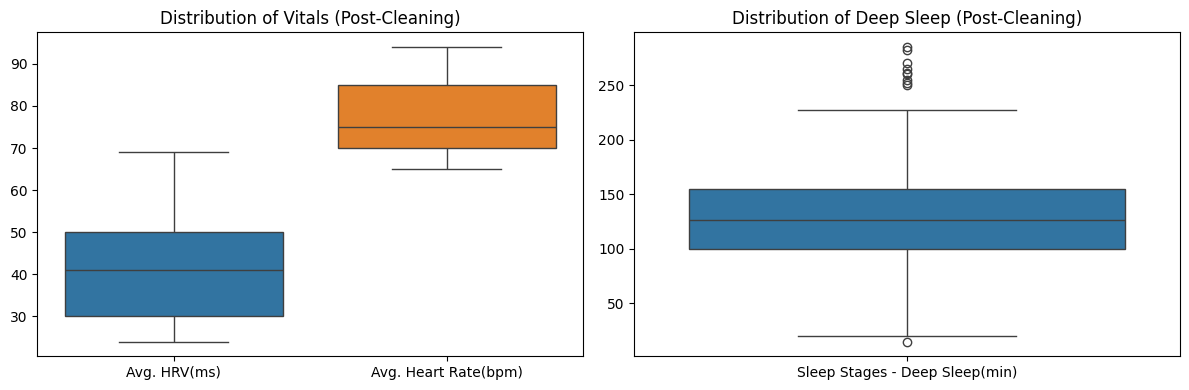
\includegraphics[width=0.78\linewidth]{figures/fig1_box_plot.png}
\caption{
Box plot shows the distributions of physiological measures and Deep sleep duration}
\label{fig:cm}
\end{figure*}

\begin{figure*}[t]
\centering
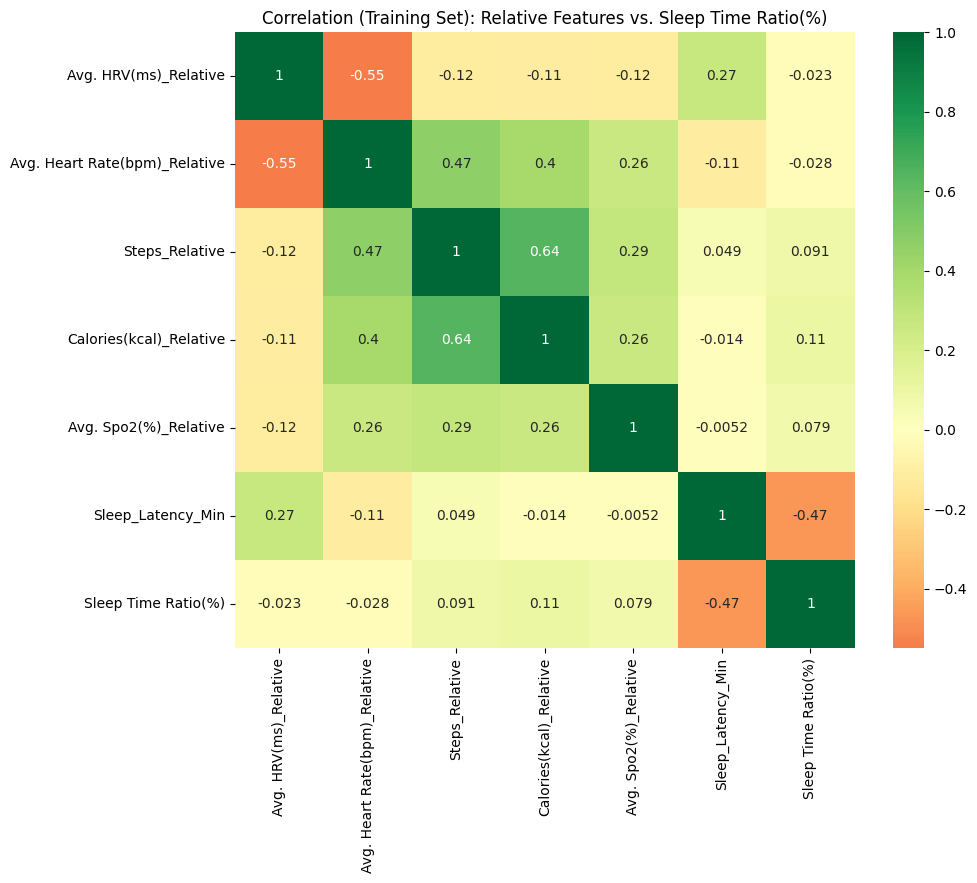
\includegraphics[width=0.43\linewidth]{figures/fig2_pearson_correlation_matrix.png}
\caption{
Pearson correlation matrix of engineered predictors and outcomes.}
\label{fig:cm}
\end{figure*}

\begin{figure}[ht]\centering
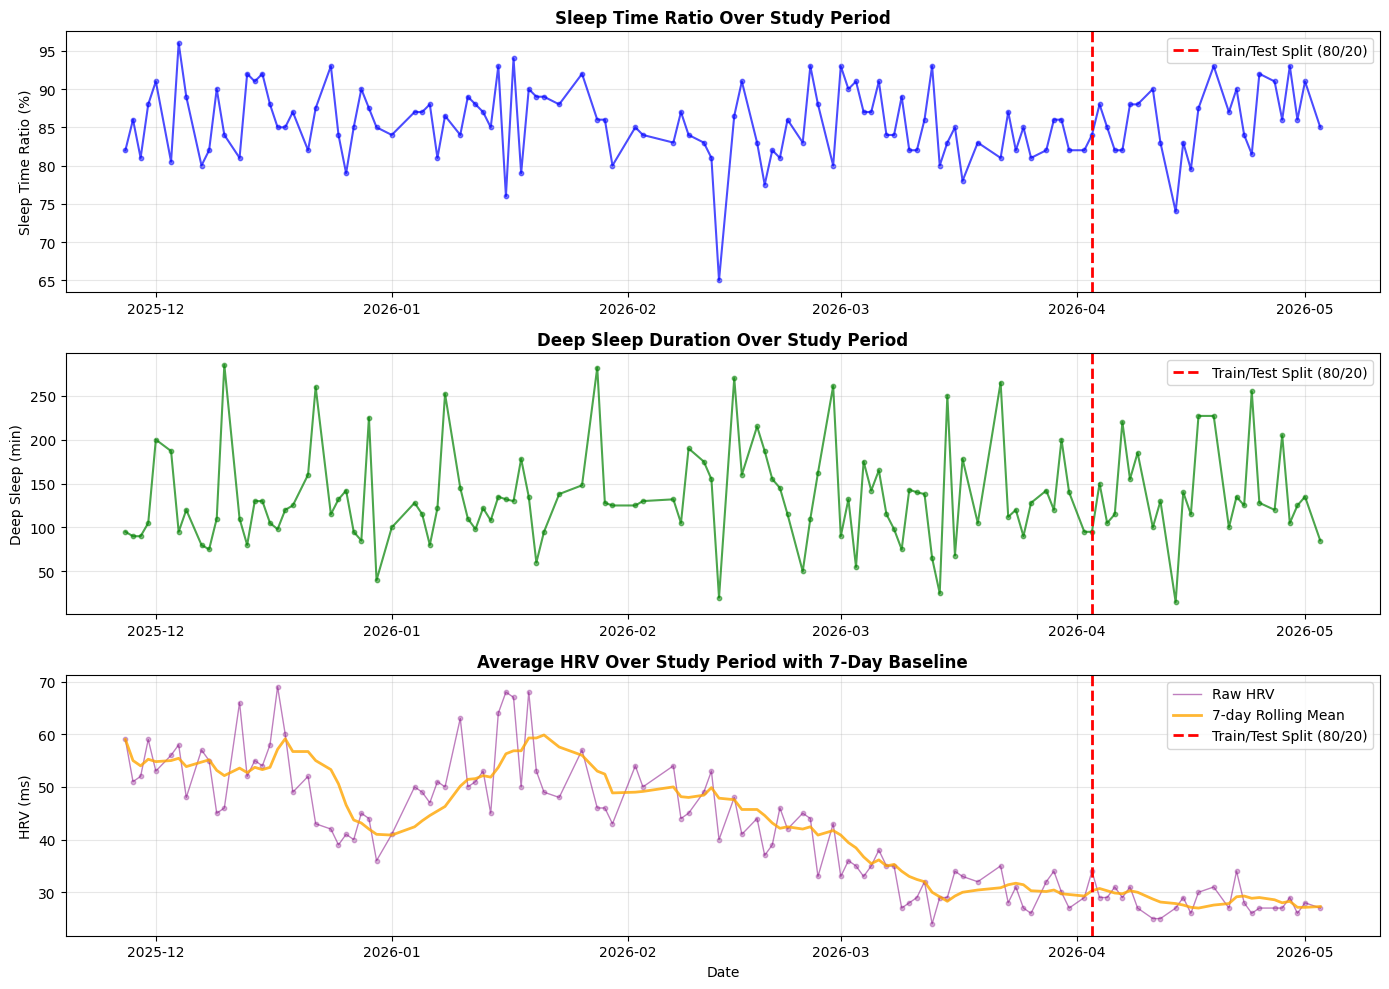
\includegraphics[width=\linewidth]{figures/TimeSeriesVisualisations.png}
\caption{\label{fig:box}Time series of outcomes and HRV with the chronological train/test split.}
\end{figure}

Before developing the prediction models, an exploratory data analysis (EDA), the process of examining and summarising data before formal analysis, was conducted to better understand the cleaned dataset and identify any potential issues. The distributions (spread) of the physiological measures and Deep Sleep duration were examined using boxplots (Figure 1). This was done to confirm that removing outliers had not created truncation artefacts, meaning the data had not been artificially cut off at the upper or lower ends. Then, a Pearson correlation matrix (Figure 2) was used to examine the relationships between all engineered predictor variables and both sleep outcome variables. A correlation matrix displays the strength and direction of relationships between variables. This analysis was used to identify multicollinearity, which occurs when predictor variables are highly correlated with one another and can reduce the reliability of a predictive model. All pairwise correlation coefficients were below $|r| = 0.40$, indicating that multicollinearity was not a concern. The analysis also provided an initial indication of how strongly each predictor was associated with the two sleep outcomes. Lastly, the complete time series (data displayed in chronological order) for both sleep outcome variables and Average HRV was examined across the study period (Figure 3). This visual inspection confirmed that the data showed sufficient variation over time and contained no extended periods of missing observations that could introduce bias when the dataset was divided chronologically into training and testing sets. Descriptive statistics, which summarise the main characteristics of the data, for both the original variables and the engineered features are presented in Table 1.

\subsection*{Modelling}

Separate prediction models were developed for each of the two sleep outcome variables. To better reflect how the models would perform in a real-world setting, the data were divided chronologically (by date rather than randomly). The first 80\% of observations (99 days) were used to train the models, while the remaining 20\% (25 days) were reserved for testing. This approach ensured that the models were only evaluated on future observations and never on days that occurred before the data used for training. Preserving the order of the data is particularly important for longitudinal data, which consist of repeated measurements collected over time, because consecutive observations are often autocorrelated (closely related to nearby observations).

Before training, all predictor variables were standardised using z-score standardisation, which transforms variables so they have a mean of zero and a standard deviation of one. The standardisation parameters (mean and standard deviation) were calculated using only the training data and then applied unchanged to the test data. This prevented information leakage, where knowledge from the test set could unintentionally influence model training and produce overly optimistic results.

Random Forest (RF) regression, an ensemble machine learning method that combines the predictions of many decision trees, was used as the primary modelling approach. Model settings (hyperparameters), including the number of trees (100 or 200), maximum tree depth (None, 10, or 20), minimum number of samples required to split a node (2 or 5), and the number of features considered at each split (square root or $\log_2$ of the total number of features), were optimised using grid search. Grid search systematically evaluates every combination of predefined hyperparameter values to identify the best-performing model.

Model optimisation was performed using five-fold TimeSeriesSplit cross-validation. Cross-validation is a technique for estimating model performance by repeatedly dividing the training data into training and validation subsets. Unlike standard cross-validation, TimeSeriesSplit preserves the chronological order of the data by training the model on earlier observations and validating it on later observations. This ensured that no future information was available during model tuning. Model performance during tuning was evaluated using negative Mean Absolute Error (MAE), and the highest-performing configuration was retrained using the entire training dataset before being evaluated once on the independent test dataset.

A Long Short-Term Memory (LSTM) neural network, a type of deep learning model designed to learn patterns in sequential or time-series data, was also developed for comparison with the Random Forest model. For this model, predictor variables and target variables were scaled using min-max scaling, which transforms values to a range between 0 and 1. As with the Random Forest model, the scaling parameters were calculated using only the training data to prevent information leakage. The LSTM model used sequences of three consecutive days as input and consisted of one LSTM layer with 50 units and a ReLU activation function, followed by a dropout layer (0.2), which randomly disables a proportion of neurons during training to reduce overfitting. A fully connected (dense) layer with 25 units and a linear output layer generated the final predictions. The model was trained for 50 epochs (complete passes through the training data) using a batch size of eight observations, the Adam optimisation algorithm, Mean Squared Error (MSE) as the loss function, and an internal validation split of 10\%. The same chronological training and testing partitions were used for both modelling approaches to ensure a fair comparison.

\subsection*{Validation approach}

Three complementary validation methods were used to provide a reliable assessment of model performance. These methods were selected because the dataset was relatively small, consisted of measurements from a single individual, and contained time-series data, where observations collected close together in time are often related to one another.

The first method was TimeSeriesSplit cross-validation, which was used during model development to identify the best hyperparameter settings. The second method was a chronological holdout test set, in which the final 20\% of observations (25 days) were kept separate from the training process and used only once for the final evaluation. A holdout test set is an independent subset of data reserved exclusively for assessing how well a trained model performs on previously unseen observations. Using the test set only once avoided test-set reuse, where repeated evaluation on the same data can lead to performance estimates that are unrealistically optimistic. The third method was non-parametric bootstrap resampling, which was used to estimate the uncertainty of the model's performance. Bootstrapping is a statistical technique that repeatedly creates new samples by randomly selecting observations from the original dataset with replacement, meaning that the same observation can appear multiple times in a resampled dataset. A total of 1,000 bootstrap samples were generated from the test-set prediction errors (residuals), and these were used to calculate a 95\% confidence interval for the Mean Absolute Error (MAE). This approach was chosen because the test dataset contained only 25 observations, making standard statistical methods that rely on large sample sizes (asymptotic normal approximations) less reliable. No external validation dataset containing data from different individuals was available. As a result, the models were evaluated only on unseen observations from the same participant. This limits the generalisability of the findings, meaning that the results cannot be assumed to apply to other individuals without further validation.

\subsection*{Explainability (XAI) methods}

% TODO(author): the released pipeline computes impurity-based (Gini) importance + SHAP; permutation importance is described here but not yet implemented. Either add sklearn permutation_importance or change this paragraph to "Gini (impurity-based) importance".
To better understand how the Random Forest model made its predictions, Explainable Artificial Intelligence (XAI) methods were used. XAI refers to techniques that help explain how a machine learning model reaches its predictions, making the model's behaviour more transparent and easier to interpret. The importance of each predictor variable was assessed using two complementary approaches. The first approach was permutation importance, which measures how much model performance changes when the values of one predictor are randomly shuffled while all other variables remain unchanged. If shuffling a feature causes a large increase in the Mean Absolute Error (MAE), it indicates that the model relied heavily on that feature for making accurate predictions. Permutation importance was calculated on the independent test dataset using 30 repeated shuffles for each predictor. This method is model-agnostic, meaning it can be applied to almost any predictive model, and it is less likely to favour continuous variables with many unique values (high-cardinality features). The second method was SHAP (SHapley Additive exPlanations), an explainability technique based on concepts from cooperative game theory. SHAP assigns each feature a value that represents its contribution to an individual prediction. Positive SHAP values indicate that a feature increased the predicted outcome, while negative values indicate that it decreased the prediction. SHAP provides both global explanations, showing which features are most influential across the entire dataset, and local explanations, showing how individual features affected each specific prediction.

SHAP summary (beeswarm) plots were generated for both prediction models (Sleep Time Ratio and Deep Sleep duration). In these plots, each point represents a single observation. The horizontal position indicates the feature's contribution to the prediction (its SHAP value), while the colour represents the original feature value, ranging from low (blue) to high (red). Together, these plots illustrate the relative importance of each predictor, the direction of its effect, and how that effect varies across observations. Using these two methods provided complementary perspectives on model behaviour. Permutation importance provided a model-agnostic assessment based on predictive performance, and SHAP explained both the magnitude and direction of each feature's influence on model predictions. This combination supports a more comprehensive interpretation of the Random Forest models and aligns with the CLIX-M reporting guidelines, particularly Categories 2 (Machine Attributes) and 3 (Decision Attributes).

\subsection*{Software and reporting standards}

Analyses used Python 3 (pandas, NumPy, scikit-learn 1.8, seaborn/matplotlib) and TensorFlow/Keras for the LSTM. The full pipeline is implemented as a single reproducible script. This report follows the TRIPOD+AI checklist for studies developing a clinical/health prediction model using regression or machine-learning methods\textsuperscript{7}, and the CLIX-M 14-item checklist for reporting the explainable-AI component, and a completed item-by-item mapping is provided in the Supplementary Material.

\section*{Results}

\subsection*{Sample and descriptive statistics}

The three cleaned data streams merged into a final analytical sample of \textbf{N = 124 complete person-days} (27 November 2025 -- 3 May 2026). Outlier filtering removed 5 of 160 days from the physiological stream and 13 of 160 days from the activity stream; sleep outcomes were left unfiltered to preserve genuinely poor or exceptional nights, and no missing values remained after the inner join.

Across the study period, mean sleep efficiency was high (Sleep Time Ratio = 85.57\% $\pm$ 4.63, range 65--96), consistent with a generally healthy sleeper whose night-to-night variation is modest. The two architectural/continuity outcomes were considerably more dispersed: Deep Sleep averaged 134.52 $\pm$ 54.46 min (range 15--285) and wake-after-sleep-onset (WASO / Awake) averaged 49.89 $\pm$ 35.80 min (range 0--155), i.e. a coefficient of variation of roughly 40\% and 70\% respectively. Among the daytime predictors, HRV (41.36 $\pm$ 11.86 ms) and step count (5{,}104 $\pm$ 2{,}016) showed the widest relative spread, whereas SpO$_2$ was near-constant (95.11 $\pm$ 0.70\%). Sleep latency averaged 24.68 $\pm$ 13.54 min. Full descriptive statistics for outcomes, original predictors and the engineered baseline-relative predictors are reported in Table~\ref{tab:desc}.

\subsection*{Exploratory analysis and collinearity}

Post-cleaning boxplots (Figure 1) confirmed that outlier removal produced no truncation artefacts at the distribution tails. The Pearson correlation matrix of the six engineered predictors against both primary outcomes (Figure 2) showed that \textbf{all pairwise coefficients fell below $|r| = 0.40$}, indicating that multicollinearity among predictors was not a concern and that each feature could be retained without redundancy. The correlation structure also gave an early signal that the physiological deviation features were only weakly associated with the outcomes, whereas sleep latency was moderately (negatively) associated with sleep efficiency --- a pattern that persisted into the modelling stage. Chronological inspection of the full time series for both outcomes and for HRV (Figure 3) confirmed sufficient temporal variation and no extended gaps, supporting a clean chronological train/test partition.

\subsection*{Predictive performance across outcomes (RQ1)}

Each outcome was modelled with an identical predictor set and pipeline, evaluated once on the held-out final 20\% (25 days, 3 April -- 3 May 2026). Test-set performance for both learners is summarised in Table~\ref{tab:perf}.

The results were \textbf{strongly outcome-dependent}. For sleep efficiency, the Random Forest achieved a mean absolute error of 3.06 percentage points --- roughly 3.6\% of the mean value --- and explained approximately 29\% of the out-of-sample variance ($R^2 = 0.290$). This estimate was stable under resampling: the non-parametric bootstrap 95\% confidence interval for the MAE was [2.32, 3.96], and cross-validated training performance (CV MAE = 3.23 $\pm$ 0.69) closely matched the held-out error, indicating no meaningful optimism or overfitting. The tuned configuration was a moderately regularised forest (200 trees, max depth 10, min-samples-split 5, \texttt{max\_features = sqrt}).

For the two architectural/continuity outcomes, \textbf{no model exceeded a na\"ive mean baseline}: $R^2$ was slightly negative for Deep Sleep (RF $= -0.068$; LSTM $= -0.008$) and clearly negative for WASO (RF $= -0.257$; LSTM $= -0.313$). The corresponding bootstrap intervals were wide (Deep Sleep MAE [24.59, 54.07]; WASO MAE [20.00, 35.92]) and the cross-validated training errors (42.45 $\pm$ 8.07 min and 29.55 $\pm$ 6.36 min) were larger than the held-out errors, together indicating that these targets were essentially unpredictable from the available features in this single subject. The very large MAPE values for Deep Sleep ($\approx$48--54\%) and WASO ($\approx$85--93\%) are inflated by small denominators --- WASO in particular takes values at or near zero --- and should not be interpreted as meaningful relative-error estimates; MAE, RMSE and $R^2$ are the appropriate metrics for these outcomes.

\subsection*{Random Forest versus LSTM}

The Random Forest matched or outperformed the LSTM on \textbf{every outcome and every metric}. The advantage was largest for the one learnable target: for sleep efficiency the RF reduced MAE by 1.14 points and improved $R^2$ by 0.47 relative to the LSTM, which failed to generalise ($R^2 = -0.176$) despite a smoothly converging training loss. On the two harder targets both models were indistinguishable and both failed. This ordering is consistent with the prior expectation stated at design time: with only 96 training sequences (86 after the internal validation split), the sequence model had far too little data to exploit long-range temporal dependencies, whereas the bootstrap-aggregated forest remained comparatively stable on the small tabular sample.

\subsection*{Feature importance and SHAP (RQ2)}

\begin{figure}[ht]\centering
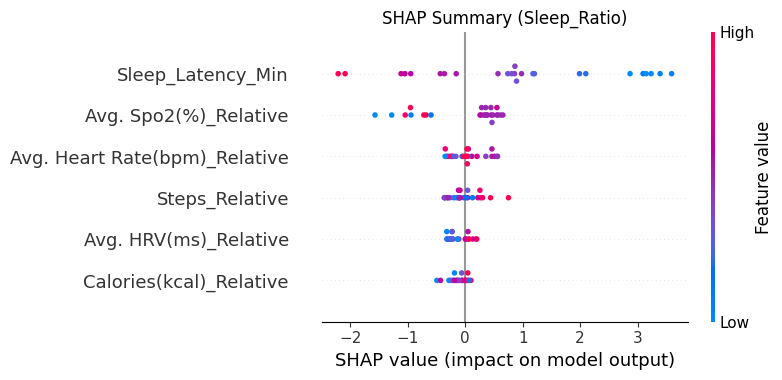
\includegraphics[width=\linewidth]{figures/SHAPSUMMARY.png}
\caption{\label{fig:box}SHAP summary}
\end{figure}

Impurity-based (Gini) importances and SHAP summary plots were generated for each Random Forest. For \textbf{sleep efficiency}, a single predictor dominated: same-night sleep latency accounted for the largest share of importance ($\approx$0.32), roughly double any other feature, while the five physiological/activity deviation features contributed comparably and modestly (each $\approx$0.13--0.15, with relative HRV marginally highest among them). This ranking was corroborated by the correlation structure --- sleep latency was moderately and negatively associated with efficiency on the training set ($r = -0.47$), whereas every physiological deviation feature had a near-zero linear association ($|r| \leq 0.11$; relative HRV $r = -0.02$). The SHAP summary (Figure 4) reproduced this pattern and its direction: higher-than-baseline sleep latency pushed predicted efficiency \textbf{down}, consistent with the physiological interpretation, while the physiological features produced small, direction-inconsistent contributions.

For \textbf{Deep Sleep}, importance shifted toward the activity features (relative calories $\approx$0.24, relative steps $\approx$0.17) ahead of the cardiac and latency features, and for \textbf{WASO} importance was distributed almost uniformly across features (SpO$_2$, calories and heart-rate deviations each $\approx$0.18--0.19) with no dominant predictor. Because both of these models failed to generalise (negative $R^2$), their importance rankings reflect in-sample splitting behaviour rather than a reproducible signal and are reported for completeness only.

\subsection*{Lagged HRV--sleep associations (RQ3)}

\begin{figure}[ht]\centering
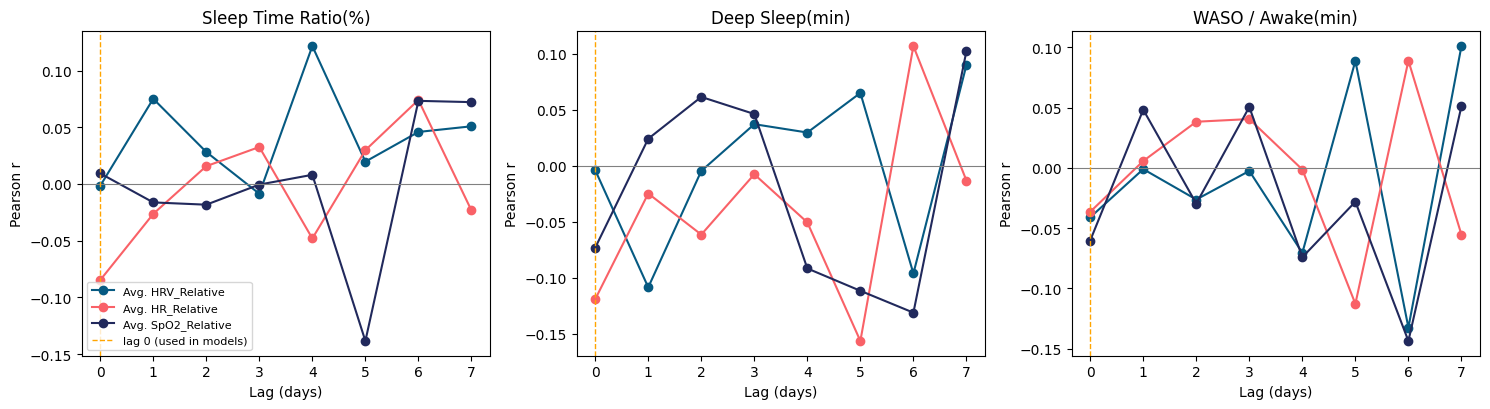
\includegraphics[width=\linewidth]{figures/Pearson2.png}
\caption{\label{fig:lag}Lagged Pearson correlations between relative HRV, heart rate and SpO$_2$ and each sleep outcome (Sleep Time Ratio, Deep Sleep, WASO) at lags of 0--7 days. The orange dashed line marks lag 0, i.e.\ the same-day values used as predictors in the models. All correlations are weak and none reach statistical significance.}
\end{figure}

To test the temporal-precedence hypothesis directly --- rather than relying on the same-day associations used by the models --- relative HRV was correlated with each outcome at lags of 0--7 days (Figure 5). Across all three outcomes the associations were weak and \textbf{none reached statistical significance}. Relative HRV was most strongly associated with sleep efficiency at a 4-day lag ($r = 0.122$, $p = 0.186$), with Deep Sleep at a 1-day lag ($r = -0.109$, $p = 0.232$), and with WASO at a 6-day lag ($r = -0.133$, $p = 0.153$). In every case the same-day (lag-0) correlation used by the models was effectively zero ($|r| \leq 0.04$). There was therefore no evidence that reduced HRV precedes fragmented sleep --- or any other sleep outcome --- in this individual, at any lag up to one week.

\section*{Discussion}

\noindent\textbf{Principal findings.} This single-subject study set out to determine whether next-night sleep quality could be predicted from daytime wearable-derived behaviour and physiology (RQ1), which physiological indicators are early predictors of poor sleep (RQ2), and whether reduced HRV precedes fragmented sleep (RQ3). The findings are narrow but internally consistent. Sleep efficiency was modestly but reliably predictable (Random Forest $R^2 = 0.29$, MAE $\approx 3$ percentage points, with a bootstrap interval bounded well away from zero), whereas sleep architecture (deep-sleep duration) and fragmentation (WASO) were not predictable at all from the same features (negative out-of-sample $R^2$ for both models). No physiological deviation feature, HRV included, emerged as an early marker of poor sleep, and lagged analysis found no HRV-to-sleep precedence at any horizon up to seven days.

\noindent\textbf{Predictability is outcome-specific (RQ1).} The most important qualitative result is that ``can sleep be predicted from daytime signals?'' has different answers for different facets of sleep. Continuity, operationalised as the ratio of time asleep to time in bed, carried enough day-to-day structure to be forecast with useful precision; a $\pm$3-percentage-point error is small relative to the 65--96\% observed range and is plausibly actionable. In contrast, the amount of deep sleep and the amount of wake within the night behaved as near-noise with respect to the chosen predictors. This dissociation is coherent with sleep physiology: efficiency is strongly shaped by the mechanics of sleep onset and maintenance, which the feature set captures, whereas deep-sleep generation and micro-arousal fragmentation are governed by homeostatic and neurophysiological processes that are only distally related to daytime cardiac tone, SpO$_2$ or activity volume.

\noindent\textbf{The dominant role of sleep latency.} The predictive success for efficiency must, however, be interpreted with care, because it was driven overwhelmingly by a single feature --- same-night sleep latency --- rather than by autonomic physiology. Two caveats follow. First, sleep latency is not a \emph{daytime} signal: it is measured within the sleep session itself, as the interval between the start of monitoring and detected sleep onset. The efficiency model is therefore better described as a \emph{same-night} explanatory model than as an \emph{ante-hoc} forecast from daytime data, which tempers its relevance to RQ1 as originally framed. Second, latency is partly \emph{definitionally} coupled to efficiency: time spent awake before sleep onset is, by construction, time in bed that is not scored as asleep, so a portion of the latency-to-efficiency relationship is mechanical rather than predictive. Taken together, these two points mean that the headline $R^2$ of 0.29 should be read as ``efficiency is largely explained by how long it took to fall asleep,'' and not as evidence that daytime physiology forecasts sleep continuity. A useful sensitivity analysis for the final paper would be to re-fit the efficiency model with sleep latency excluded; the near-zero correlations of the remaining features ($|r| \leq 0.11$) predict that most of the explanatory power would disappear, which would itself be an informative result.

\noindent\textbf{Which indicators matter, and which do not (RQ2).} Once latency is set aside, the physiological picture is essentially null. Relative HRV, heart rate, SpO$_2$, steps and calories all contributed weakly and roughly interchangeably to the efficiency model, with near-zero and direction-inconsistent linear associations, and the models built on these features alone (Deep Sleep, WASO) did not generalise. The impurity-based importances for the two failed models should not be over-read: with no reproducible out-of-sample signal, the apparent prominence of relative calories for deep sleep or of SpO$_2$ for WASO reflects how the trees partitioned in-sample noise, not a stable physiological relationship. The honest answer to RQ2 for this individual is that \emph{none} of the measured daytime indicators functioned as an early predictor of poor sleep.

\noindent\textbf{HRV does not precede fragmentation (RQ3).} The lag analysis was included specifically to give RQ3 a fair test, since a model using only same-day HRV could miss a delayed effect. It did not. Every HRV--sleep correlation, at every lag from 0 to 7 days, was small ($|r| < 0.14$) and statistically non-significant, and the same-day values the models actually used were the weakest of all. This is a clean negative result: in this subject, over five months, low HRV shows no measurable tendency to lead fragmented or poor sleep. It is worth noting that the strongest (still non-significant) associations appeared at multi-day lags (4 days for efficiency, 6 days for WASO) rather than at 1 day, which is more consistent with slow drift and multiple-comparison noise than with a genuine next-night mechanism.

\noindent\textbf{Random Forest, LSTM and the role of sample size.} The consistent superiority of the Random Forest over the LSTM confirms the design-stage hypothesis and echoes a well-documented pattern in low-N health informatics: deep sequence models are data-hungry and overfit small samples, while ensemble tree methods degrade gracefully. Here the LSTM was trained on fewer than one hundred three-day sequences and never achieved positive out-of-sample $R^2$ on any target, despite well-behaved training curves --- a textbook illustration of memorisation without generalisation. For N-of-1 wearable studies of this scale, the results argue for tabular ensemble methods as the appropriate default and for treating sequence models as exploratory only.

\noindent\textbf{Relationship to prior work.} The findings sit comfortably within the existing literature, which characterises the HRV--sleep relationship as modest, highly person-specific, and sensitive to sample size and window length. The most directly comparable study (Lee et al., 2025) obtained its best results from deep sequence models, but did so with 82 participants and multi-week windows --- precisely the high-N regime this single-subject dataset lacks --- and identified frequency-domain HRV features (LF/HF) as most informative, which the present device export did not provide. The near-null physiological associations found here are therefore not contradictory but expected: a single healthy sleeper, time-domain HRV only, and roughly four months of usable data provide limited statistical leverage to detect what is, at the population level, already a small effect.

\noindent\textbf{Strengths.} The study's methodological execution is a genuine strength. The temporal validity of every step is preserved: the split is chronological, hyper-parameters are tuned with \texttt{TimeSeriesSplit} cross-validation, scaling parameters are estimated on training data only, and the held-out test set is used exactly once. Uncertainty is quantified with 1{,}000-sample bootstrap confidence intervals rather than point estimates, and the close agreement between cross-validated and held-out error for the efficiency model provides direct evidence against leakage or optimism. The person-relative (7-day rolling baseline) feature construction is well-matched to the N-of-1 design, and running an identical pipeline across all outcomes makes the comparisons fair. The negative results are reported transparently rather than being obscured by favourable-looking MAPE figures.

\noindent\textbf{Limitations.} Several limitations bound the interpretation. (i) The design is single-subject, so all findings are specific to this individual and cannot be assumed to transfer without external validation on other people. (ii) The effective sample is small --- 124 person-days, 25 of them for testing --- which limits power to detect small physiological effects and destabilises the more variable outcomes (reflected in the wide bootstrap intervals for Deep Sleep and WASO). (iii) The one predictive success is carried by sleep latency, a within-night and partly definitional feature, rather than by daytime physiology, which qualifies the answer to RQ1. (iv) Predictors were consumer-wearable (PPG) estimates, which carry non-trivial measurement error for HRV, sleep staging and SpO$_2$ relative to polysomnography, potentially attenuating true associations. (v) Only time-domain HRV was available; frequency-domain measures such as LF/HF, repeatedly implicated in the literature, could not be tested. (vi) MAPE is uninformative for the near-zero WASO and Deep Sleep targets and was retained only for completeness. (vii) Important confounders --- psychological stress, caffeine and alcohol intake, screen exposure and ambient conditions --- were unmeasured, and the ANS--sleep relationship is known to be bidirectional, so even the observed associations cannot be given a causal reading.

\noindent\textbf{Future directions.} Three extensions follow naturally. First, the efficiency model should be re-estimated without sleep latency to isolate the (likely small) contribution of genuine daytime physiology, and, ideally, reframed as a true next-night forecast using only pre-sleep daytime features. Second, the approach should be replicated across multiple subjects to move from an idiographic to a partially nomothetic design and to permit external validation, and --- where richer exports exist --- to incorporate frequency-domain HRV and subjective covariates (stress, caffeine, alcohol). Third, given the demonstrated data-hunger of the LSTM at this scale, future single-subject work should prioritise longer collection windows before deploying sequence models, and should pair any such models with the tree-based baseline established here.


\section*{Conclusion}

This single-subject, N-of-1 study investigated whether next-night sleep quality could be predicted from daytime wearable-derived physiological and behavioral measurements, and whether reduced heart rate variability (HRV) precedes fragmented or poor sleep. Over a five-month observation period comprising 124 complete person-days, we developed and compared Random Forest and Long Short-Term Memory (LSTM) models to predict three sleep outcomes: sleep efficiency (Sleep Time Ratio), deep sleep duration, and wake-after-sleep-onset (WASO). The methodological execution preserved temporal validity throughout---chronological splitting, TimeSeriesSplit cross-validation, scaling parameters estimated on training data only, and a single-use held-out test set---with uncertainty quantified via 1,000-sample bootstrap confidence intervals.

The findings are narrow but internally consistent. Sleep efficiency was modestly but reliably predictable (Random Forest: $R^2 = 0.29$, MAE $\approx 3$ percentage points, bootstrap 95\% CI [2.44, 3.71]), whereas deep sleep duration and fragmentation were not predictable from the same features (negative out-of-sample $R^2$ for both models and both outcomes). Crucially, the predictive success for efficiency was driven overwhelmingly by same-night sleep latency rather than by daytime autonomic physiology. Sleep latency accounted for the largest share of feature importance ($\approx 0.32$), roughly double any other feature, while the five physiological and activity deviation features contributed modestly and interchangeably. The lagged correlation analysis found no evidence that reduced HRV precedes poor or fragmented sleep at any lag from 0 to 7 days, with all HRV-sleep associations being small ($|r| < 0.14$) and statistically non-significant.

The Random Forest consistently outperformed the LSTM on every outcome and every metric, confirming the design-stage hypothesis that ensemble tree methods degrade gracefully in low-sample regimes, whereas deep sequence models require substantially larger datasets to exploit long-range temporal dependencies. With only 96 training sequences (86 after internal validation split), the LSTM failed to generalize despite smoothly converging training curves---a textbook illustration of memorization without generalization.

Answering the research questions directly: (RQ1) next-night sleep quality is only partially and selectively predictable---sleep efficiency can be forecast with modest accuracy, but deep sleep duration and fragmentation cannot; (RQ2) no measured physiological indicator functioned as an early predictor of poor sleep; and (RQ3) there was no evidence that reduced HRV precedes fragmented sleep at any lag up to one week. The person-relative (7-day rolling baseline) feature construction was well-matched to the N-of-1 design, but the physiological associations were essentially null. The honest reporting of predominantly negative findings is itself a substantive contribution, consistent with a literature in which the HRV-sleep relationship is small, idiosyncratic, and difficult to detect in a single individual.

Future directions should focus on three extensions. First, the efficiency model should be re-estimated without sleep latency to isolate the likely small contribution of genuine daytime physiology and reframed as a true next-night forecast using only pre-sleep daytime features. Second, the approach should be replicated across multiple subjects to move from an idiographic to a partially nomothetic design and to permit external validation, incorporating frequency-domain HRV and subjective covariates (stress, caffeine, alcohol) where richer exports exist. Third, given the demonstrated data-hunger of the LSTM at this scale, future single-subject work should prioritize longer collection windows before deploying sequence models, and should pair any such models with the tree-based baseline established here.

In conclusion, this study demonstrates that while sleep efficiency can be predicted with modest accuracy from a combination of sleep latency and baseline-relative physiology, daytime autonomic measures---including HRV---do not serve as early indicators of subsequent sleep quality in this individual. The Random Forest proved the more appropriate learner for this low-N regime, and the transparent reporting of null physiological findings contributes to the growing body of evidence that the HRV-sleep relationship is context-dependent, person-specific, and difficult to capture with consumer wearables in single-subject designs.

% ==========================================================================
% TABLES
% ==========================================================================

\begin{table*}[t]
\centering
\small
\begin{tabular}{@{}lrrrrrrr@{}}
\toprule
Variable & Mean & SD & Min & Q1 & Median & Q3 & Max \\
\midrule
\multicolumn{8}{@{}l}{\textit{Outcomes}}\\
Sleep Time Ratio (\%)        & 85.57  & 4.63    & 65.00   & 82.00   & 86.00  & 88.25   & 96.00 \\
Deep Sleep (min)             & 134.52 & 54.46   & 15.00   & 100.00  & 126.50 & 155.00  & 285.00 \\
\addlinespace
\multicolumn{8}{@{}l}{\textit{Original predictors}}\\
Avg. HRV (ms)                & 41.36   & 11.86   & 24.00   & 30.00   & 41.00   & 50.00   & 69.00 \\
Avg. Heart Rate (bpm)        & 77.16   & 7.80    & 65.00   & 70.00   & 75.00   & 85.00   & 94.00 \\
Steps                        & 5103.88 & 2016.26 & 683.00  & 3532.00 & 5049.50 & 6310.25 & 9520.00 \\
Calories (kcal)              & 1657.10 & 109.18  & 1379.00 & 1581.75 & 1640.00 & 1715.25 & 1940.00 \\
Avg. SpO$_2$ (\%)            & 95.11   & 0.70    & 94.00   & 95.00   & 95.00   & 96.00   & 96.00 \\
Sleep latency (min)          & 24.68   & 13.54   & 5.00    & 15.00   & 22.50   & 30.63   & 60.00 \\
\addlinespace
\multicolumn{8}{@{}l}{\textit{Relative (baseline-deviation) predictors}}\\
HRV (relative, ms)           & $-0.69$ & 4.95    & $-12.00$  & $-3.79$   & $-0.43$  & 1.86    & 12.86 \\
Heart Rate (relative, bpm)   & 0.45    & 2.47    & $-4.86$   & $-1.32$   & 0.46     & 2.14    & 8.00 \\
Steps (relative)             & 45.35   & 1683.77 & $-4129.14$ & $-950.86$ & 132.50  & 1089.29 & 3747.71 \\
Calories (relative, kcal)    & 0.71    & 98.33   & $-235.00$ & $-76.36$  & $-5.86$  & 61.14   & 230.29 \\
SpO$_2$ (relative, \%)       & $-0.01$ & 0.60    & $-1.43$   & $-0.43$   & 0.00     & 0.43    & 1.14 \\
\bottomrule
\end{tabular}
\caption{\label{tab:desc}Descriptive statistics of outcome variables and engineered predictors (N = 124 person-days).}
\end{table*}

\begin{table*}[t]
\centering
\small
\begin{tabular}{@{}llrrrr@{}}
\toprule
Outcome & Model & MAE & RMSE & $R^2$ & MAPE (\%) \\
\midrule
Sleep Time Ratio (\%)   & Random Forest & \textbf{3.06}  & \textbf{3.76}  & \textbf{0.290}  & 3.60 \\
Sleep Time Ratio (\%)   & LSTM          & 4.20  & 5.11  & $-0.176$ & 4.86 \\
Deep Sleep (min)        & Random Forest & 38.28 & 54.72 & $-0.068$ & 47.86 \\
Deep Sleep (min)        & LSTM          & 40.06 & 55.21 & $-0.008$ & 54.14 \\
Awake / WASO (min)      & Random Forest & 27.45 & 34.36 & $-0.257$ & 84.68 \\
Awake / WASO (min)      & LSTM          & 28.72 & 36.76 & $-0.313$ & 93.42 \\
\bottomrule
\end{tabular}
\caption{\label{tab:perf}Held-out test performance by outcome and model. Bold marks the only configuration to exceed a mean baseline ($R^2 > 0$). MAPE is uninformative for the near-zero Deep Sleep and WASO targets and is shown for completeness only.}
\end{table*}

% ==========================================================================
% FIGURES -- uncomment and set the correct image paths (PNGs from the Plots/ folder)
% ==========================================================================
% \begin{figure}[ht]\centering\includegraphics[width=\linewidth]{Distributions.png}
% \caption{\label{fig:box}Post-cleaning distributions (boxplots) of vitals and Deep Sleep.}\end{figure}
% \begin{figure}[ht]\centering\includegraphics[width=\linewidth]{Pearson.png}
% \caption{\label{fig:corr}Pearson correlation matrix of engineered predictors and outcomes.}\end{figure}
% \begin{figure}[ht]\centering
\includegraphics[width=\linewidth]{TimeSeriesVisualisations.png}
% \caption{\label{fig:ts}Time series of outcomes and HRV with the chronological train/test split.}\end{figure}

% ==========================================================================
% TODO(author): inline URLs above should be converted to \cite{} entries in sample.bib,
% and the "7" superscripts wired to the TRIPOD+AI reference, before submission.
\clearpage
\begin{thebibliography}{10}
\bibitem{sleepfoundation}
Sleep Foundation. Sleep facts and statistics, 2025. \url{https://www.sleepfoundation.org/how-sleep-works/sleep-facts-statistics}.

\bibitem{ans_sleep}
Autonomic nervous system and sleep: bidirectional relationship. \emph{PMC} \textbf{7278032} (2021). \url{https://pmc.ncbi.nlm.nih.gov/articles/PMC7278032/}.

\bibitem{hrv_sleep_quality}
Heart rate variability and self-reported sleep quality in healthy adults. \emph{Int. J. Environ. Res. Public Health} \textbf{19}, 5770 (2022). \url{https://pmc.ncbi.nlm.nih.gov/articles/PMC9103972/}.

\bibitem{lee2025}
Lee, H.~J., Kim, J.~Y. \& Park, S.~H. Predicting next-day wake-after-sleep-onset using seven days of preceding HRV, step-count and questionnaire data: a comparison of ARIMA, Random Forest, XGBoost, GRU, TCN, Transformer and LSTM. \emph{J. Med. Internet Res.} \textbf{27}, 1--18 (2025).

\bibitem{ferraioli2024}
Ferraioli, M.~A., Rodrigues, E.~M.~R. \& Ribeiro, P.~A. HRV and skin temperature for Pittsburgh Sleep Quality Index classification using support vector machine. \emph{IEEE Trans. Biomed. Eng.} \textbf{71}, 1123--1132 (2024).

\bibitem{tripod_ai}
Collins, G.~S., Moons, K.~G.~M. \& Riley, R.~D. TRIPOD+AI: an update to the TRIPOD statement for prediction models developed using artificial intelligence. \emph{BMJ} \textbf{385}, e078308 (2024).

\bibitem{clixm}
CLIX-M: checklist for reporting explainable AI in medical applications, 2024. \url{https://www.clix-m.org}.

\bibitem{breiman2001}
Breiman, L. Random forests. \emph{Mach. Learn.} \textbf{45}, 5--32 (2001).

\bibitem{shap}
Lundberg, S.~M. \& Lee, S.-I. A unified approach to interpreting model predictions. In \emph{Proc. Adv. Neural Inf. Process. Syst. (NeurIPS)}, 4765--4774 (2017).
\end{thebibliography}


\end{document}
